\documentclass{article}
\usepackage{graphicx}

\begin{document}

\title{Visual Exploration of Climate Data, Using Icon-Annotated Maps}
\author{Cook, Hofmann, Wickham, Wickham, Cheng}

% Drawing trend lines on map
%   - How to
%   - Comparison to coloring slope
%   - Reference to Grinstein icon plots
% Pickett RM and Grinstein GG (1988). Iconographics 
% displays for visualizing multidimensional data. 
% In Proc. IEEE Conference on Systems, Man, and Cybernetics, pages 514-19.
% Note the later work on metaphoric data display, garbage work!
%   - Alexander Gribov's work http://rosuda.org/software/Gauguin/gauguin.html

% Interactive graphics
% Data processing

% Perhaps the GHCN data? Not gridded
% NOAA data, almost grid, but over ocean, so maps more tricky
% NARCAP from NCAR?
% Fill in with NASA data, to start, try to put new data for final version

\maketitle

\section{Introduction}

Need a colorful map, facetted by year \& month

\begin{figure*}[htp]
\includegraphics[width=6in]{images/nasa-colored-map.png}
\caption{Facetted map of de-seasonalized temperature.}
\end{figure*}

\section{Generating a time series at each location}

\begin{figure*}[htp]
\centerline{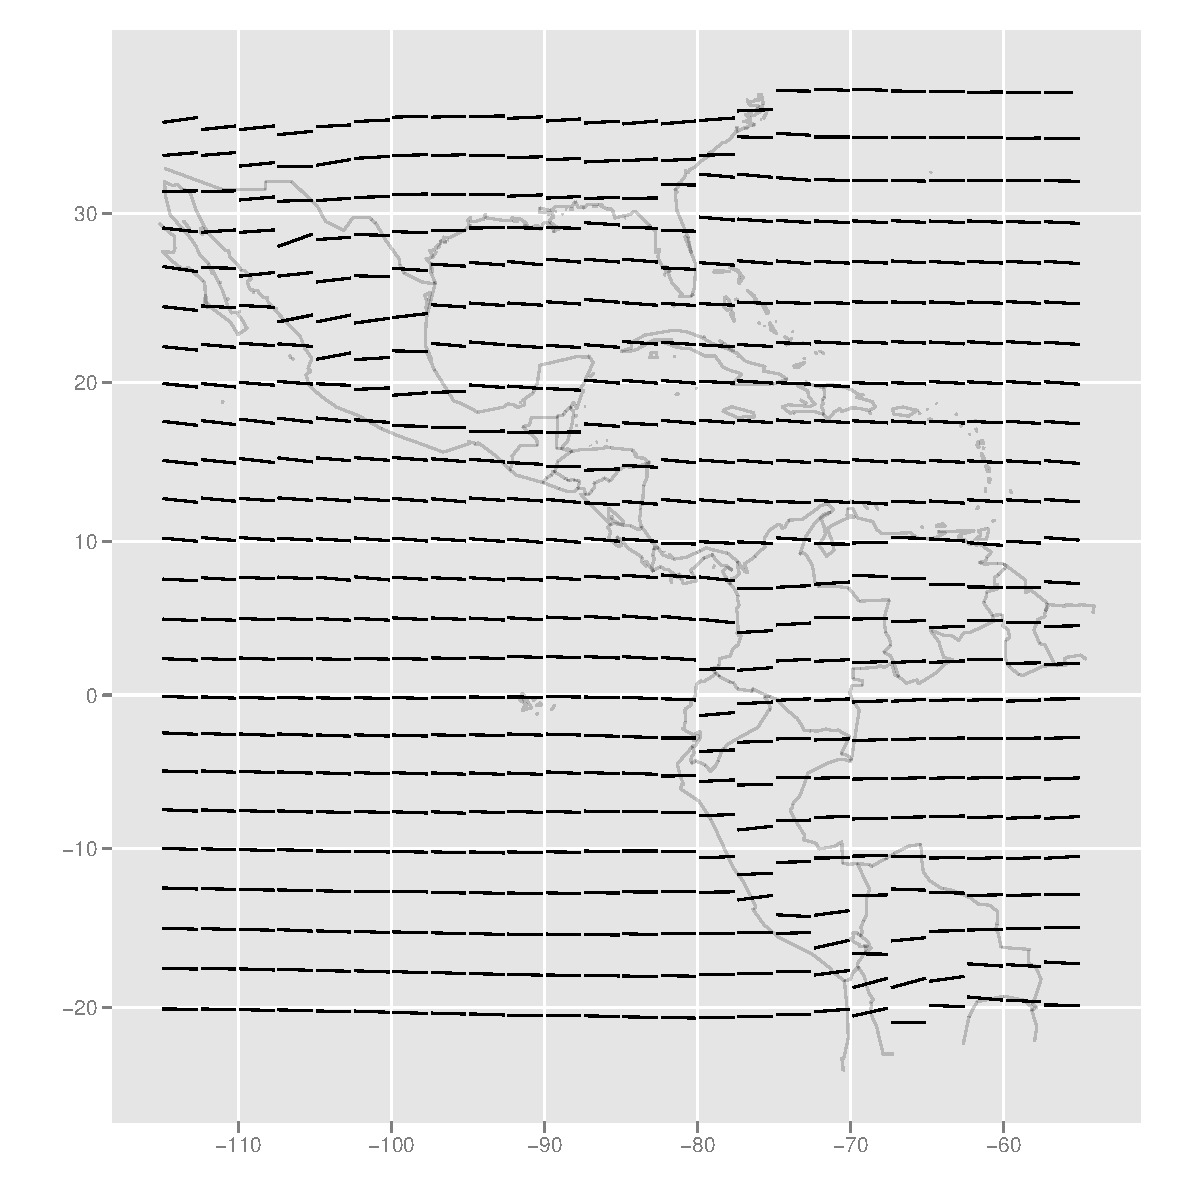
\includegraphics[width=4in]{images/nasa-deseas-trend.pdf}}
\caption{Time series icon at each location, showing de-seasonalized trend.}
\end{figure*}

\section{Showing seasonal effect, radially oriented icon}

\section{Effect of scale}

\section{Reference lines and boxes}

\section{Regular vs irregular locations}


\end{document}